% !TEX encoding = UTF-8
% !TEX TS-program = pdflatex
% !TEX root = ../../tesi.tex

\section{Smart contract per HotMoka}
Lo \textit{smart contract} per HotMoka ha il compito di gestire gli NFT generati dalla piattaforma NFTLab nella \textit{blockchain} HotMoka.

\subsection{Progettazione}
La progettazione del contract per la \textit{blockchain} HotMoka è molto simile a quella che è stata eseguita per il contratto per Ethereum. Le differenze principali sono ovviamente nelle convezioni date dal linguaggio, infatti Takamaka segue le stesse convezioni di linguaggio che da Java. 
I \textit{design pattern} che ho utilizzato sono gli stessi, ovvero il \textbf{\textit{Access Restriction}} e il \textbf{\textit{Guard Check}}.

\begin{figure}[h!]
  \centering
  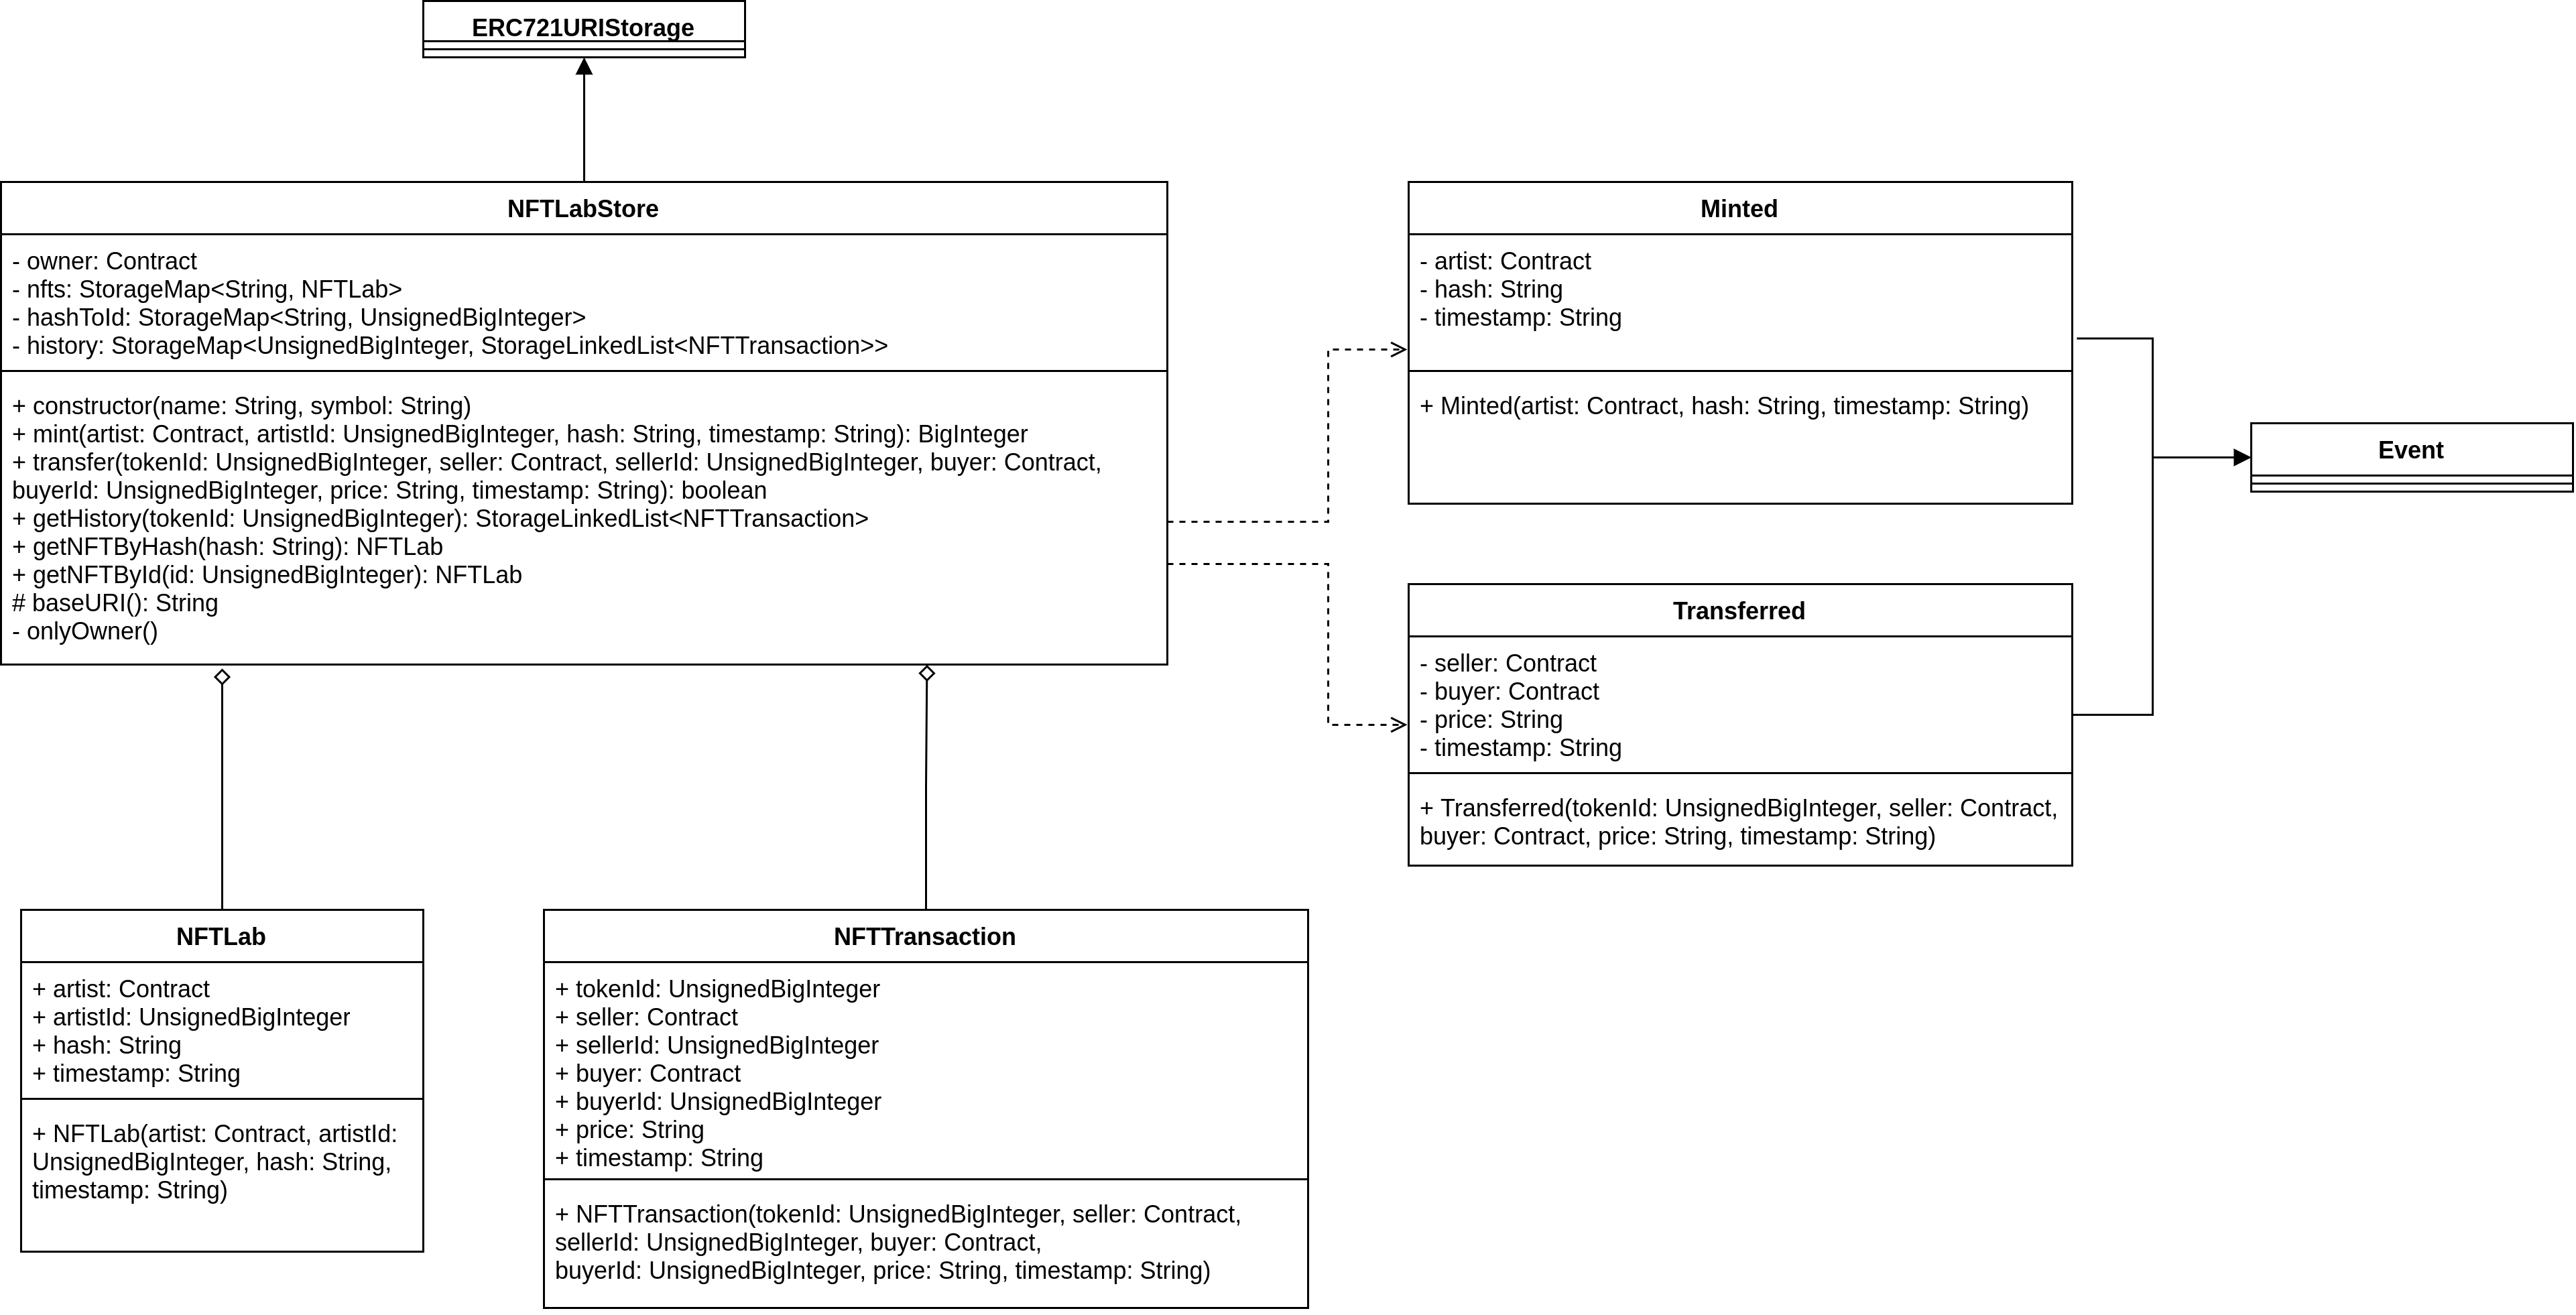
\includegraphics[width=\textwidth]{capitolo3/class-diagram/smart-contract-hotmoka-class-diagram.png}
  \caption{Diagramma delle classi dello \textit{smart contract} per HotMoka}
\end{figure}

\subsection{Codifica}
In seguito alla fase di progettazione, sono passato alla codifica. Anche qui ho prima scritto tutta la struttura di quanto dovevo sviluppare, ovvero classi e firme dei metodi, per poi solo in seguito passare alla scrittura del corpo.

Le principali differenze con il linguaggio Solidity, che si possono notare anche in fase di progettazione, sono la non presenza di determinati costrutti al livello del linguaggio. Infatti Takamaka non presenta delle sintassi che facilitano l'utilizzo degli eventi e dei modificatori.

\begin{figure}[h!]
  \centering
  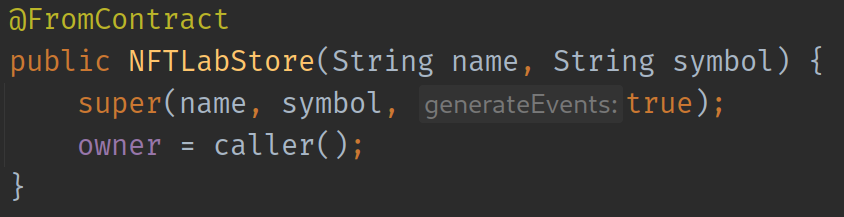
\includegraphics[width=0.8\textwidth]{capitolo3/smart-contract-hotmoka/smart-contract-hotmoka-constructor.png}
  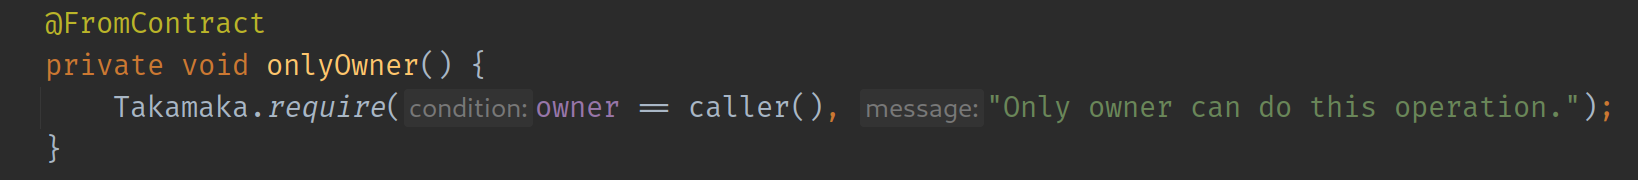
\includegraphics[width=0.8\textwidth]{capitolo3/smart-contract-hotmoka/smart-contract-hotmoka-modifier.png}
  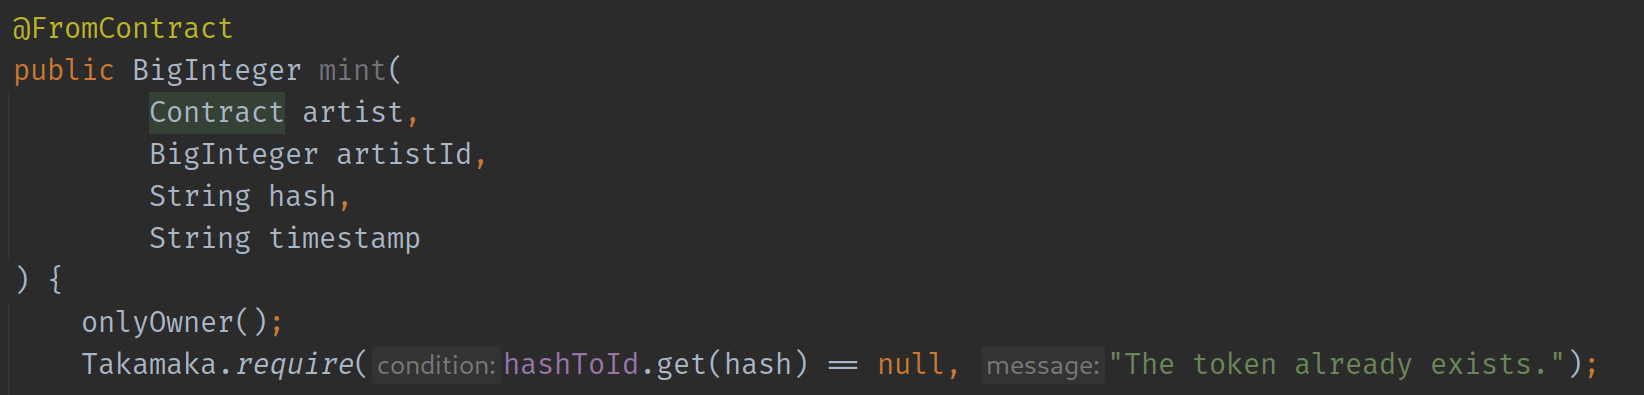
\includegraphics[width=0.8\textwidth]{capitolo3/smart-contract-hotmoka/smart-contract-hotmoka-modifier-usage.png}
  \caption{Realizzazione del \textit{design pattern Access Restriction} in Takamaka}
\end{figure}

\subsection{Verifica}
In parallelo con l'attività di codifica, ho verificato lo sviluppo del contratto sfruttando il \textit{framework} \textbf{JUnit5} e la libreria \textbf{TakamakaTest}. Questi ultimi si integrano perfettamente con lo strumento Maven. Dato che lo \textit{smart contract} può essere eseguito solamente su \textit{blockchain}, TakamakaTest provvederà ad eseguire il \textit{deploy} di quest'ultimo in una \textit{blockchain} temporanea dove verranno eseguiti tutti i \textit{test}. 

Per quanto riguarda i tipi di test eseguiti, gli unici che sono stati sviluppati sono quelli di unità, perché non potevano essere sviluppati altri tipi di \textit{test} per la natura semplice delle funzioni.

\begin{figure}[h!]
  \centering
  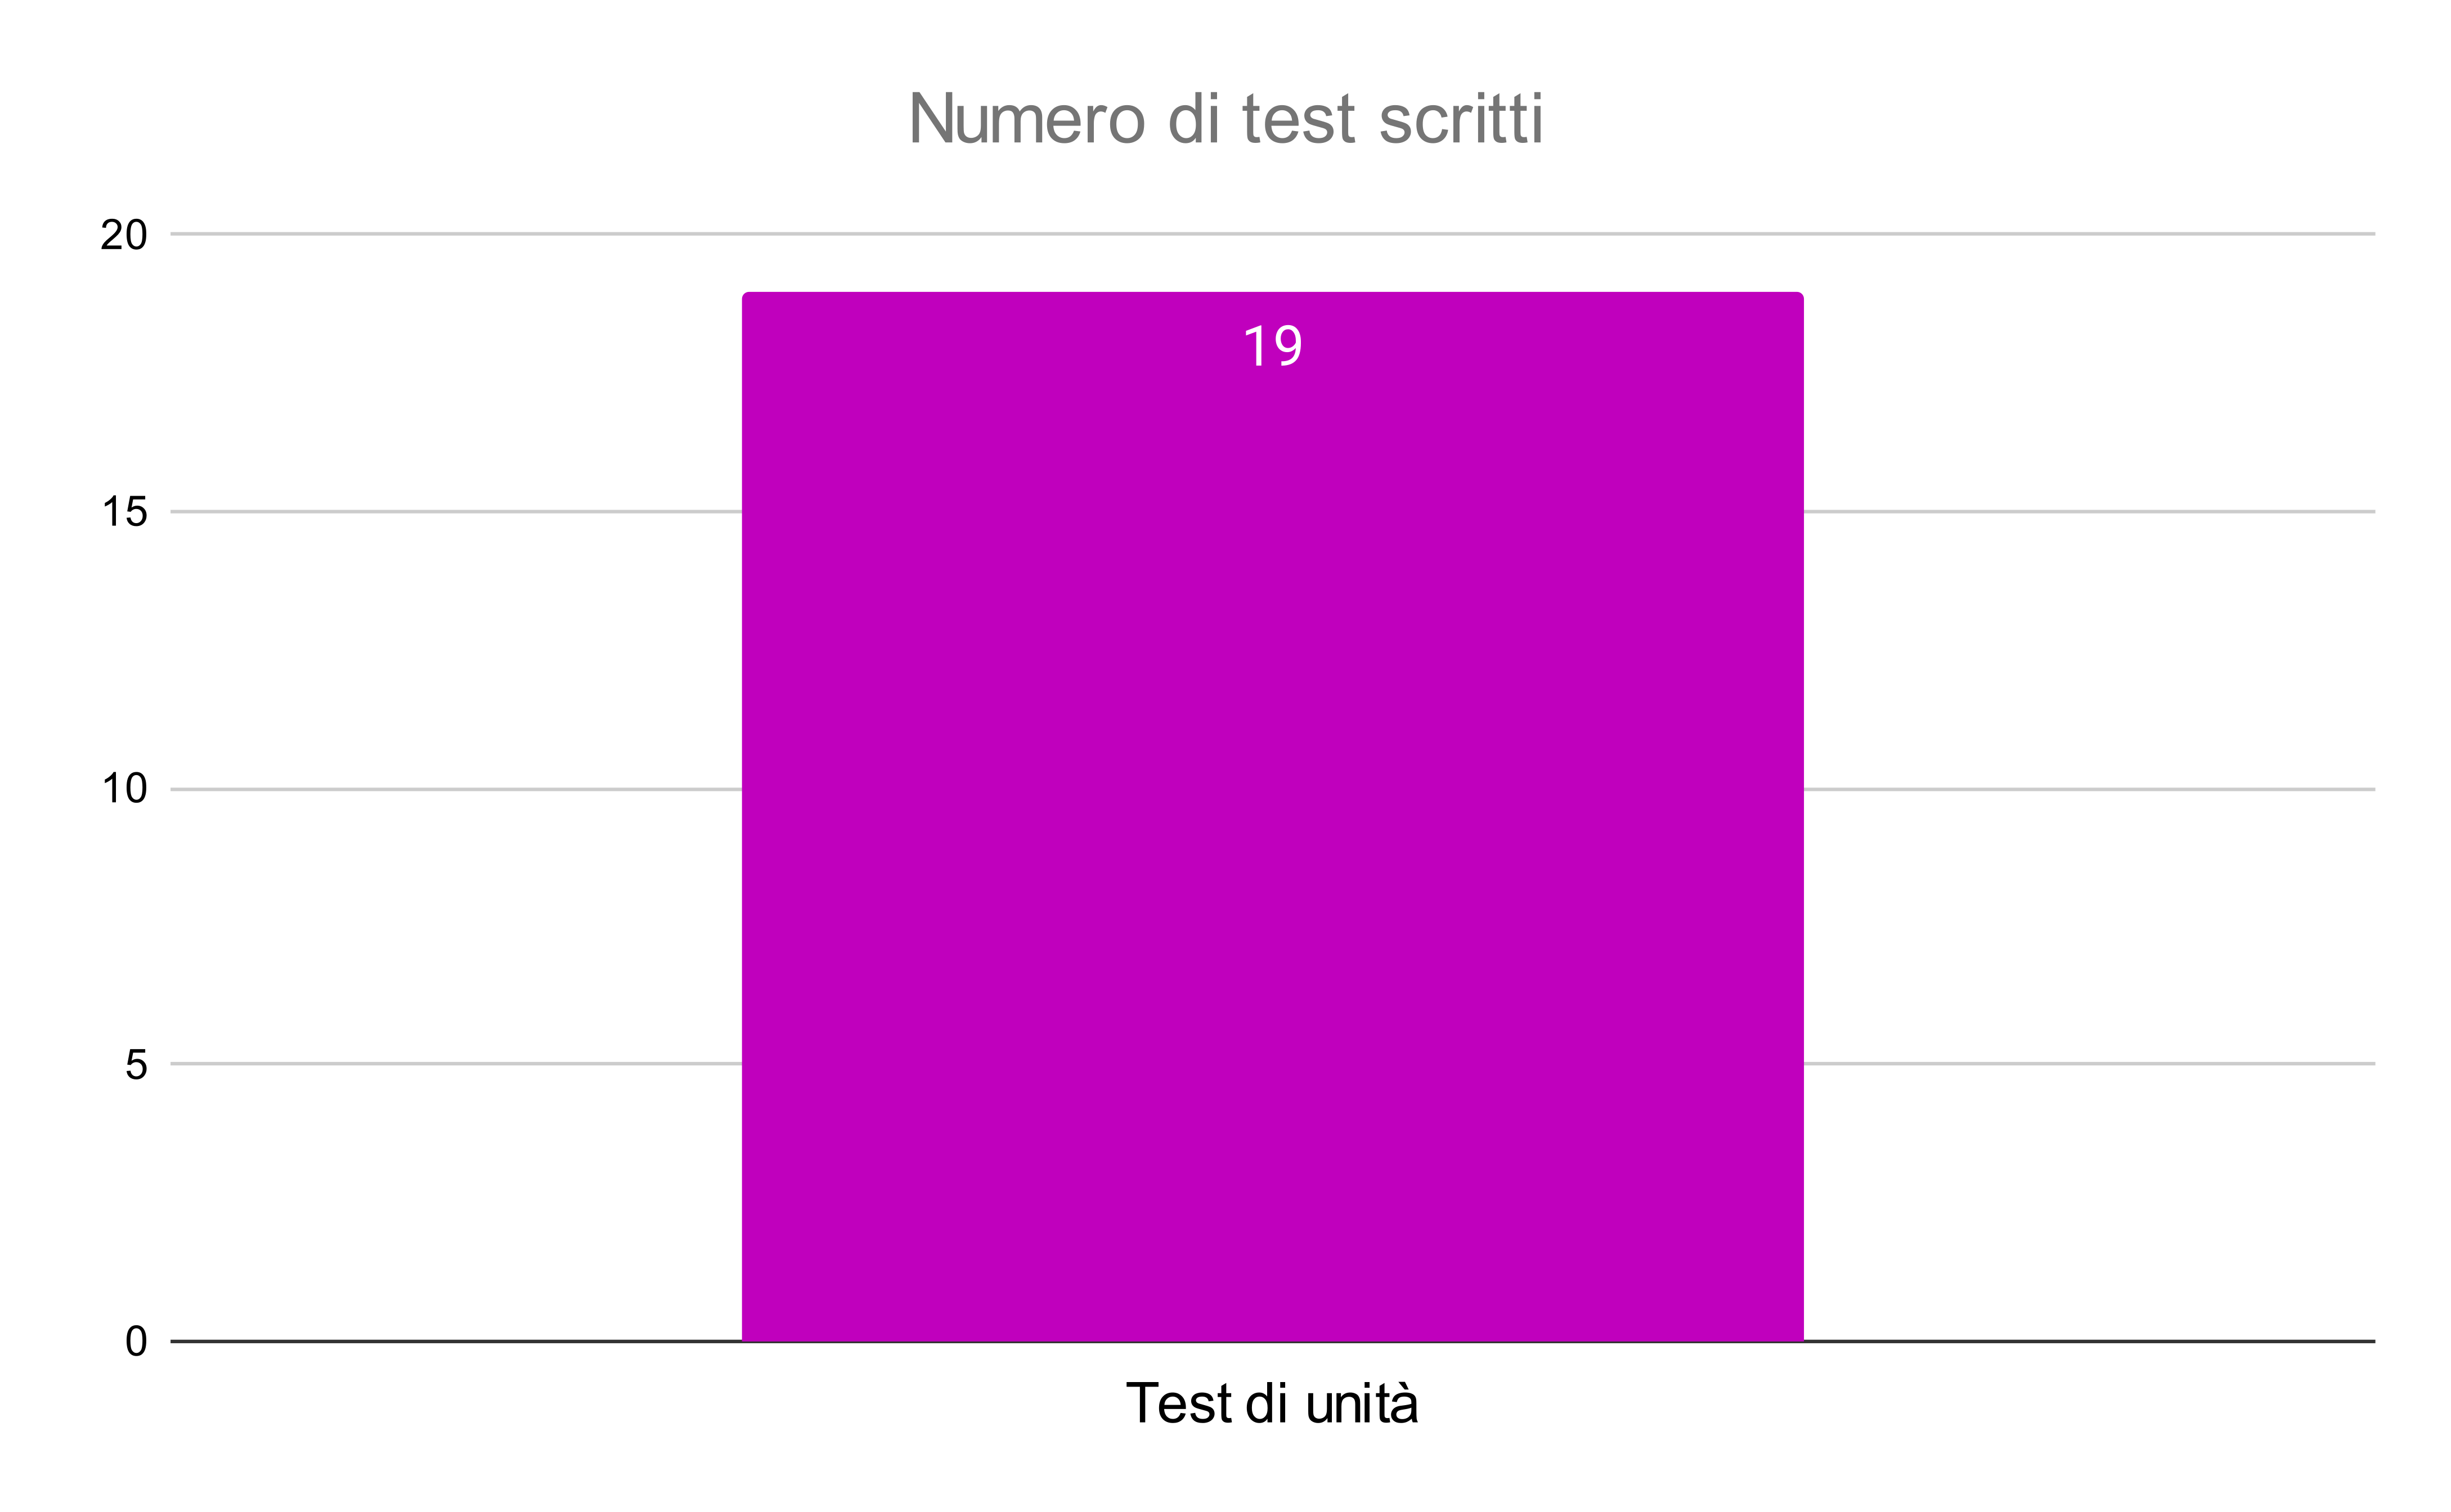
\includegraphics[width=0.8\textwidth]{capitolo3/smart-contract-number-test.png}
  \caption{Numero di test scritti nel contratto in HotMoka}
\end{figure}

In generale, posso affermare che l'attività di verifica si è rilevata molto proficua e mi ha permesso di agevolare lo sviluppo in modo significativo, tanto da produrre un grande quantitativo di \textit{test} e raggiungere un \textit{code coverage} del 100\%.

% \clearpage
\begin{figure}[h!]
  \centering
  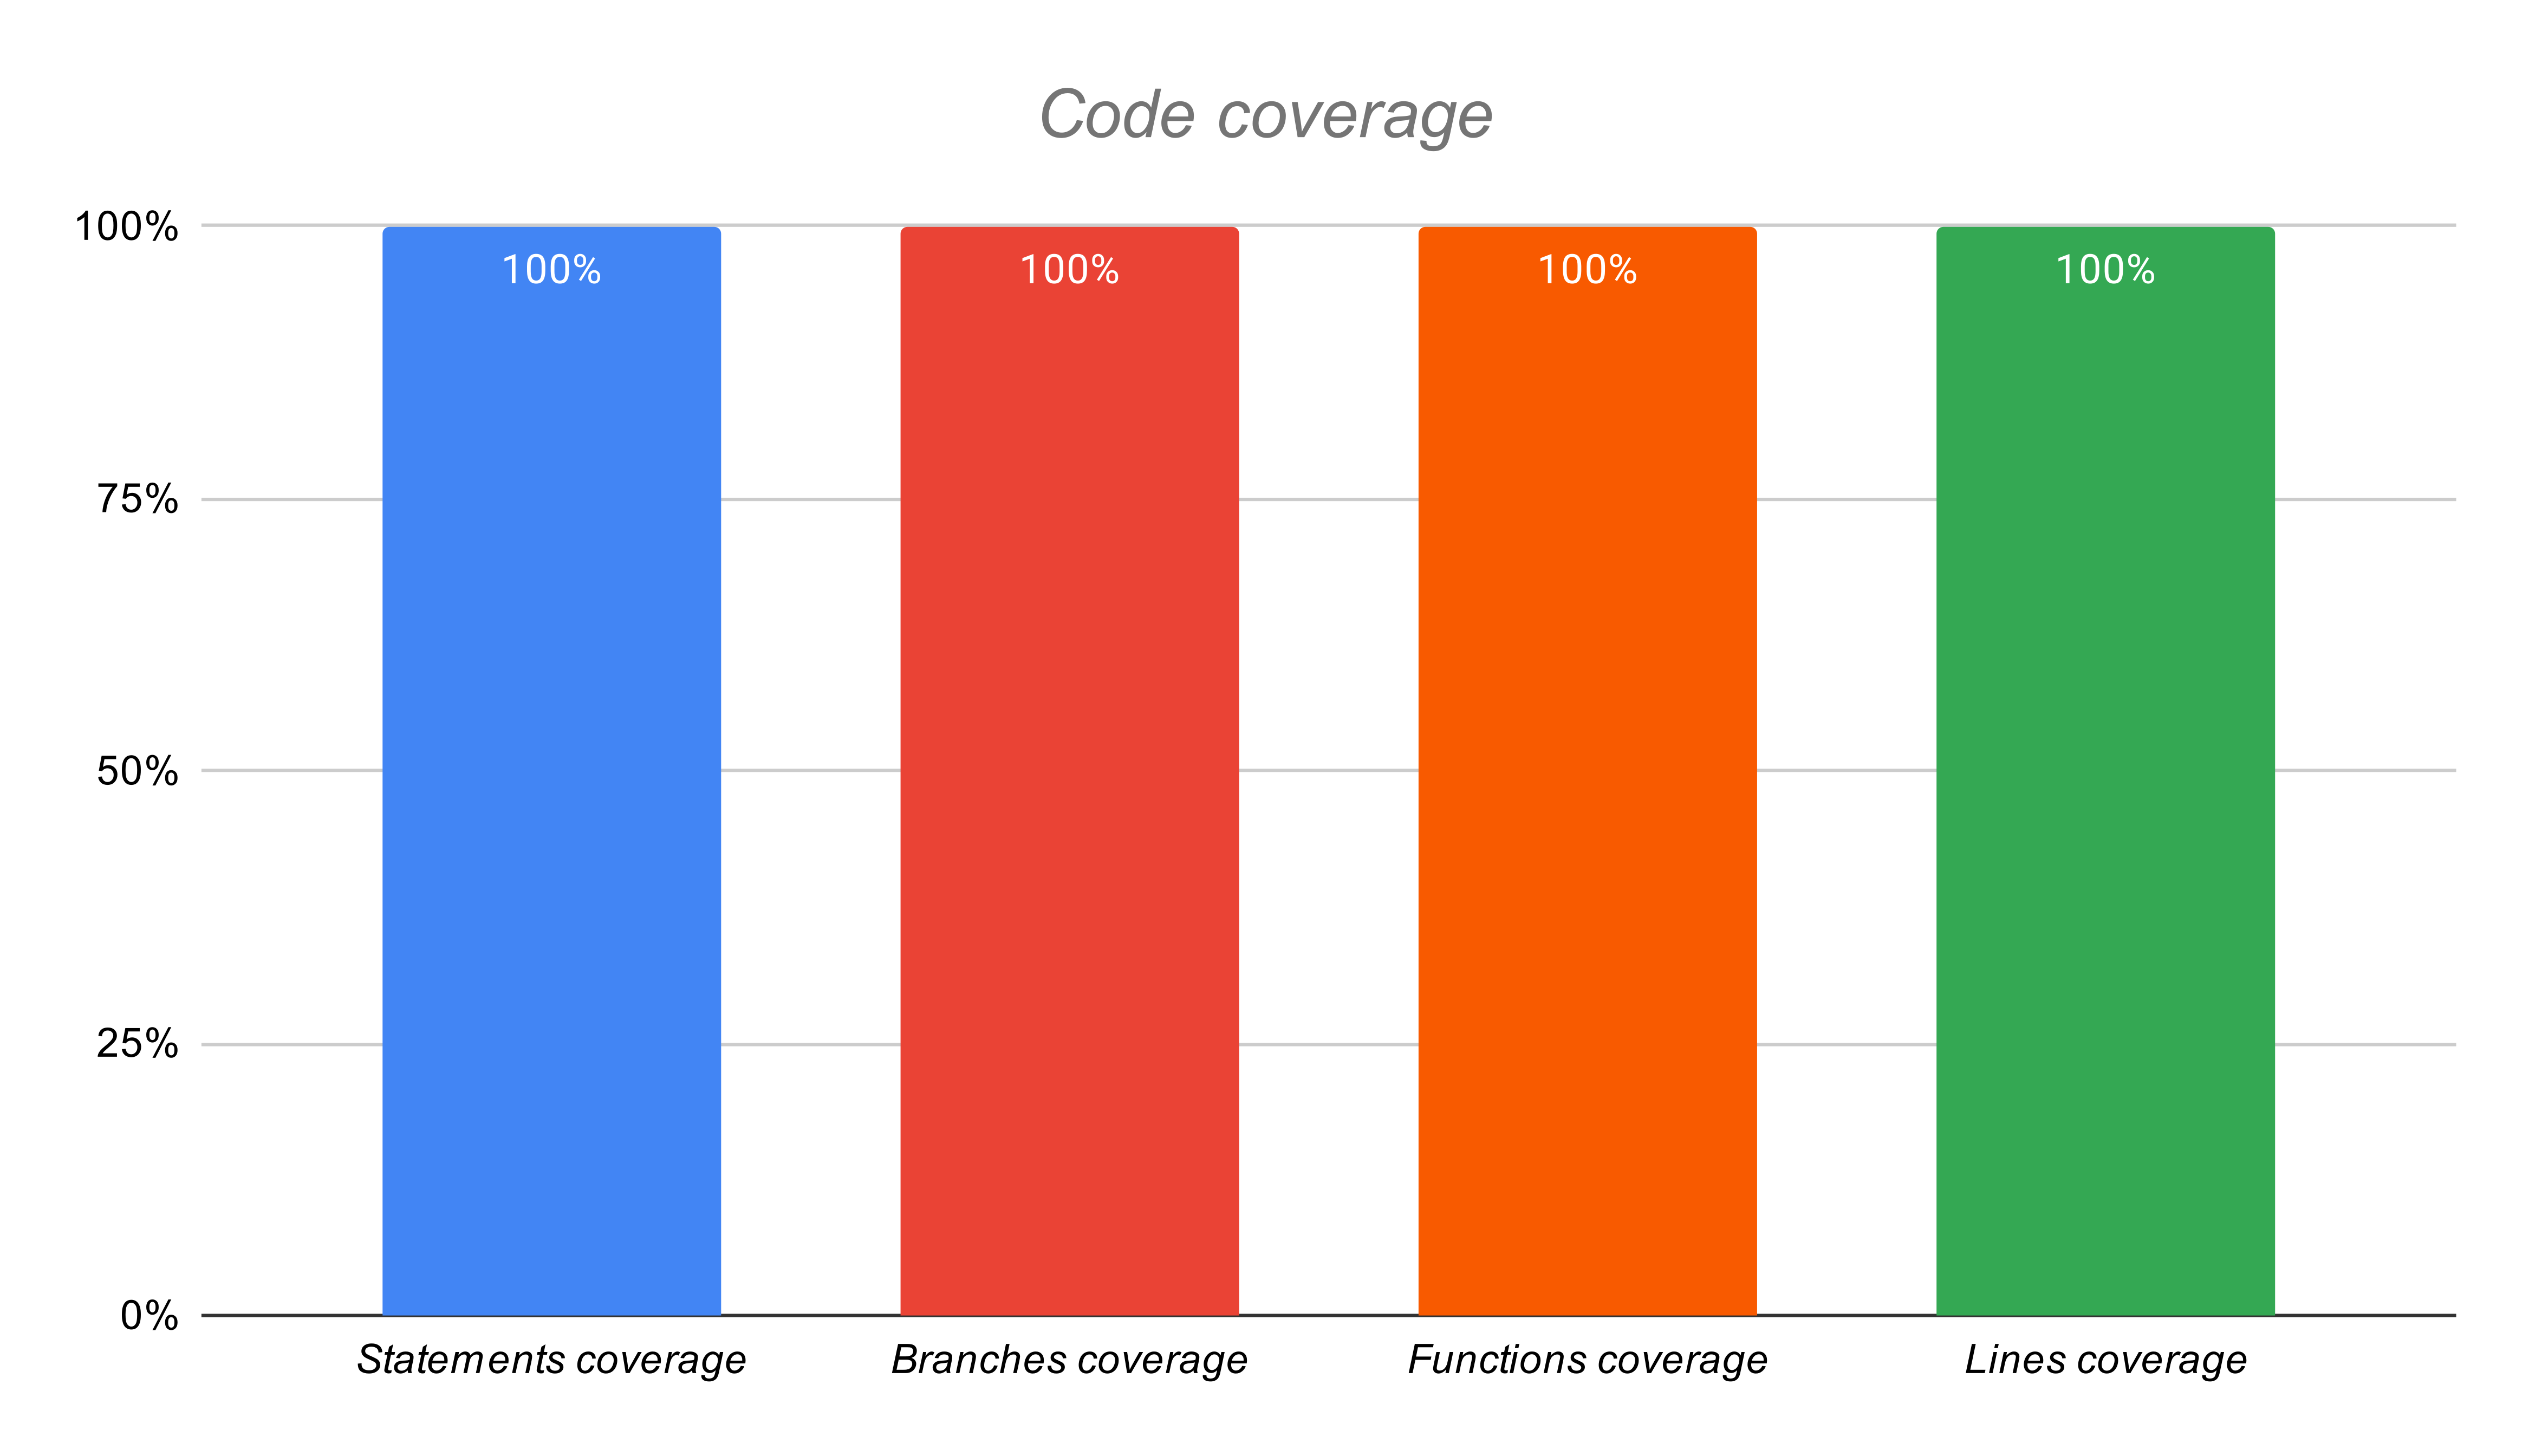
\includegraphics[width=0.8\textwidth]{capitolo3/smart-contract-code-coverage.png}
  \caption{\textit{Code coverage} raggiunto nel contratto in HotMoka}
\end{figure}
